\documentclass[../BTOF_summary.tex]{subfiles}
 
\begin{document}

\section{The \btof\ Detector Hardware}

The \btofD\ consists of 16 elements arranged symmetrically around the \panda\ interaction point. Each of these elements is called a \sm\ and comprises four main parts.

\begin{itemize}
	\item Active Medium (Scintillator Tiles)
	\item Photon Readout (\sipm)
	\item Signal Transmission (PCB / \railboard )
	\item Enclosure (Carbon Fiber)
\end{itemize}

A single large PCB or a PCB split into a front and back part connect the Front End Electronics (FEE) to the detector elements. 
Each \sm\ is equipped with 60 scintillator tiles in two rows, read out by four \sipms\ on each side of the scintillator. 
This adds up to 3840 channels with a total amount of \num{15360} deployed \sipms .

\subsection{Scintillator}
Each scintillator of the \btofD\ is identical to the others and have the following dimensions; \SI{87 x 29.4 x 5}{mm}.
To fit inside the holding structure the corners of the scintillator tiles are truncated.
Each chamfer is set at \SI{3}{mm}.
This is a change from the design proposed in the Technical Design Report (TDR) which had rectangular scintillators.

The performance impact of this change was studied using a strontium source on a mechanized arm, comparing time resolution measurements of cut and uncut scintillator tiles.\todo[inline]{The measurements of Svetlana need to be integrated here}
As shown in \fig\ \todo{add figure} the bulk of the material shows little to no significant difference.
The time resolution of events in the corners... \todo{finish this paragraph}

\subsubsection*{Material}
The scintillator of choice for the detector dimensions is the EJ-232 by Eljen Technology. It is an organic scintillator compound developed for high accuracy timing applications \footnote{\url{https://eljentechnology.com/products/plastic-scintillators/ej-232-ej-232q}}.
The equivalent Saint-Gobain/Bicron equivalent product would be the BC-422 scintillator.
Another material candidate was the widely used EJ-228/BC-418.
It produces more photons but for the small dimensions of the \btof\ tiles delivers a slightly inferior time resolution.
%Due to the short emission wavelength the mean free path inside of the scintillator is only around \SI{10}{cm}.

Measurements comparing the scintillator thickness revealed stark differences in performance between \SI{3}{mm} and \SI{6}{mm} thick tiles. 
Under ideal circumstances, for equal readout surface and constant energy loss of passing particles, the number of detected photons is independent of the thickness.
However, since the number of internal reflections is increased for thinner tiles, more photons are lost at the scintillator surface compared to thicker modules.
This leads to a significant time resolution increase when reducing the tile thickness as can be seen in \fig ~\ref{fig:Tchickness_timeRes}.
Since the performance difference between \SIlist[]{5;6}{mm} is minimal and the material budget of the device needs to be kept at a minimum the detector will be equipped with \SI{5}{mm} thick tiles.

\begin{figure}[htbp]
	\centering
	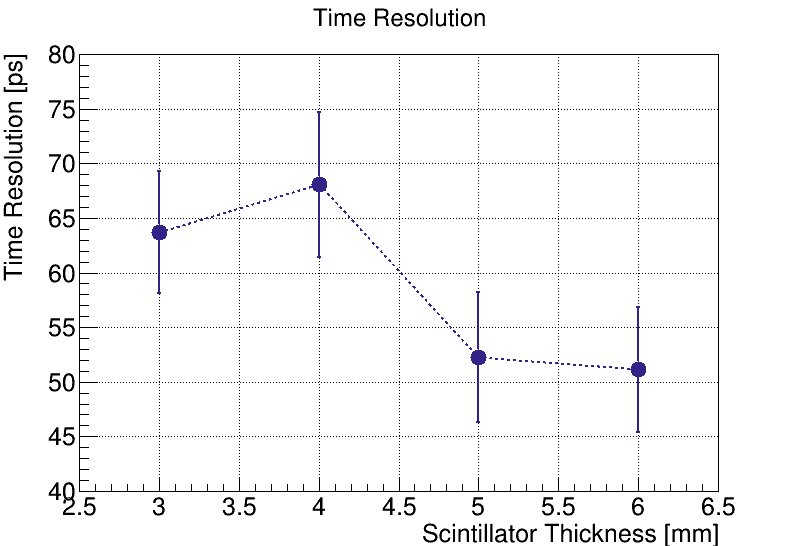
\includegraphics[width=.7\textwidth]{fig/TimeResSummary.png}
	\caption{Time resolution measurement comparing different thicknesses of aluminized mylar wrapped scintillator tiles.}
	\label{fig:Tchickness_timeRes}
\end{figure}

\subsubsection*{Wrapping}
Since the time resolution of a scintillator detector is coupled to the number of detected photons, the scintillator tiles are wrapped in order to reflect photons that escape the scintillator back into it.
The material choice was subject to tests performed on a scintillator tile using a \sr\ source in order to determine the best performing wrapping.
Material candidates were aluminized mylar foil, Tyvek hardstructure 1057D, enhanced specular reflector (ESR), Teflon tape, aluminum foil and no wrapping.
As can be seen in Table~\ref{tab:WrappingTest}, taken from the \btof\ TDR\todo[]{add Ref to TDR}, the performance difference was within \SI{6.7}{ps} from the best to the worst performing wrapping and a standard deviation of \SI{2.23}{ps}.

\begin{table*}[htbp]
	\caption[Time resolution for different wrapping materials]{Time resolution of EJ-232 (top) and EJ-228 (bottom) plastic scintillator tiles for various wrapping materials.
		\label{tab:WrappingTest}}
	\centering
	%\resizebox{0.8\textwidth}{!}
	{
		\begin{tabular}{ l  c  c }
			\toprule
			Wrapping material                 & Time resolution [ps] & Number of detected photons \\
			\midrule
			No wrapping                       & 55.0\,$\pm$\,0.3     & 288\,$\pm$\,2\\
			Aluminized Mylar foil             & 52.7\,$\pm$\,0.3     & 355\,$\pm$\,2\\
			Tyvek hardstructure 1057D         & 55.0\,$\pm$\,0.3     & 394\,$\pm$\,3\\
			Enhanced specular reflector (ESR) & 55.2\,$\pm$\,0.3     & 355\,$\pm$\,3\\
			Teflon tape                       & 59.4\,$\pm$\,0.3     & 408\,$\pm$\,4\\
			Aluminum foil                     & 54.2\,$\pm$\,0.3     & 344\,$\pm$\,3\\
			\midrule
		\end{tabular}
	}
\end{table*}

Surprisingly, Teflon tape, the by far worst performing wrapping, produced the largest amount of detected photons.
The best performing material and the only one better than no wrapping at all was the aluminized mylar foil.
This can be attributed to the type of reflection.
While aluminized mylar has a mirror like finish, the other materials produce diffuse reflections.
This leads to larger distances travelled by the photons before reaching the photo detectors.

The wrapping material of choice for the scintillator tile of the \btofD\ is aluminized mylar.


\subsection{\sipm}

To detect the photons produced in the scintillators a device is needed that fits into the limited space available to the detector, can operate within a strong magnetic field and delivers a good time resolution.
A sensor that fits these criteria is the Silicon Photomultiplier (\sipm ).
These small devices are available in multiple sizes.
Best suited for the \btofD\ is an effective photosensitive area of \SI{3x3}{mm} with a thickness in the order of \SI{1.5}{mm}.

Multiple manufacturers offer sensors of such kind including \hamamatsu, \ketek and \advansid\ each with slightly different operational parameters.
One main point to consider is the operational voltage which differs greatly between manufacturers.
While \hamamatsu\ \sipms\ are operated at around \SI{60}{V}, \ketek\ \sipms\ only require a bias voltage of around \SI{30}{V}.
Since the sensors will be connected in series as described in Section \todo{add section on SiPM serial connection}, the operational voltage is 4 times the single sensor voltage, which affects the requirements from necessary electronics to drive the sensors.

The final choice on which \sipm\ model to use has not been made since the development of \sipms\ moves relatively fast and new product generations were expected.
Tested sensors include the \texttt{S13360-3050PE} by \hamamatsu, the \texttt{PM3350} by \ketek\ and the \texttt{ASD-NUV3S-P} by \advansid , which all perform adequately.

\subsubsection*{Serial connection of 4 \sipms}

In order to effectively readout the \SI{5x30}{mm} large surface area of the ends of the scintillator tile, the active surface needs to be extended beyond a single \sipm\ with an effective photosensitive are of \SI{3x3}{mm}.
To do this four \sipms\ are connected in series.
This offers a larger active area without increasing the detector complexity by adding unnecessary channels by reading out the \sipms\ individually.

Additionally connecting the sensors in series in contrast to a parallel connection, offers an improvement of the signal timing properties.
The slope of the rising signal flank, which determines the signals timing susceptibility to electrical noise, depends on the sensors internal capacitance.
A smaller capacitance leads to a faster sensor discharge and a steeper signal slope.
Connecting the sensors in series decreases this internal capacitance making the signal faster whereas a parallel connection would have the opposite effect.

There is evidence suggesting, that increasing the amount of \sipms\ from 4 to 6 would improve the time resolution.
These tests however were performed at a time where the scintillator was held in place differently and hence was not chamfered.
Cutting away \SI{3}{mm} from either edge reduces the available space to \SI{24}{mm}.
With the actual width of each \sipm\ is slightly below \SI{4}{mm} and an LED between the middle two sensors, there simply is not enough room for additional sensors.

\subsection{\railboard}

The solution to connect the photo sensors to the FEE and provide mechanical support at the same time is the \railboard .
It is a long PCB split into two parts due to availability issues of the base material.

Previous designs relied solely on the mechanical support of a single \railboard\ spanning the entirety of a \sm\ to hold all components including the scintillators in place.
Due to stability issues and too small tolerances in the connectors the form of the board has been redesigned and a carbon frame has been added.
The single \railboard\ is replaced by four large PCB's, one of which is shown in \fig ~\ref{fig:Railboard}.
Two of these boards are connected by ribbon cables to connect one full row of 60 scintillators to the FEE.

\begin{figure}
	\centering
	\includegraphics*[width=.9\textwidth]{fig/Railboard3_imageCombined.png}
	\caption{Combined depiction of the internal transmission line layout and a photograph of the front part of the \railboard .}
	\label{fig:Railboard}
\end{figure}

\sipm\ signals with a rise time of \SI{3}{ns} correspond to a frequency of \SI{167}{MHz}.
At this frequency dielectric losses start to take on a larger portion of the electric losses experienced along a transmission line\footnote{more information in the dissertation of S. Zimmermann}.
To reduce these losses special PCB substrate materials have been developed such as RO4003C by Rogers Corp.
This is the material that is used for the \btof\ \railboard\ to ensure minimal losses for an optimal performance.



\end{document}